\chapter{Planificación}
En está sección vamos a explicar y desglosar varios aspectos relativos a la organización y desarrollo del proyecto como pueden ser sus etapas, la metodología empleada, herramientas de productividad y herramientas de desarrollo.

\section{Metodología usada}
La metodología que hemos empleado para el desarrollo de la aplicación es una de las pertenecientes al grupo de las \textit{ágiles}, cuyo nombre es \textbf{``SCRUM''}. 

La principal característica de ``SCRUM'' es la división del proyecto en otros más pequeños, cada uno de los cuales con sus propias etapas de análisis, diseño, desarrollo, etc. Dentro de la etapa de desarrollo se producen los denominados ``sprints'', que consisten, a grandes rasgos, en realizar regularmente entregas de una parte del proyecto para ser evaluadas.

Algunas de las ventajas que podemos obtener gracias al uso de esta metodología son la flexibilidad, la falta de grandes errores arrastrados por un desarrollo largo y una mayor libertad e innovación propiciados por el continuo planteamiento del proyecto\cite{VanessaRosello}.

Aplicado al desarrollo de nuestra aplicación, esto se traduce en la división del software en diferentes partes, cada una de las cuales se prueba con distintos usuarios a medida que se va completando. De este modo, es posible comprobar rápidamente qué partes del proyecto son más problemáticas y cuáles ofrecen mejores resultados, así como obtener una opinión general de los usuarios que puede y debe ser utilizada para guiar y replantear a tiempo múltiples partes del mismo. 

\section{Organización del proyecto}

\subsection{Etapas del proyecto}
\begin{itemize}
  \item \textbf{1ª etapa:} Estudio del problema.
  \item \textbf{2ª etapa:} Aprendizaje en Android.
  \item \textbf{3ª etapa:} Análisis de requisitos.
  \item \textbf{4ª etapa:} Planificación del proyecto.
  \item \textbf{5ª etapa:} Diseño de software e interfaz.
  \item \textbf{6ª etapa:} Implementación.
  \item \textbf{7ª etapa:} Pruebas.
  \item \textbf{8ª etapa:} Documentación.
\end{itemize}

Entre las etapas listadas anteriormente, aquellas que van desde la tercera hasta la séptima (ambas inclusive), se repetirán para cada una de las partes en las que estará dividido el desarrollo de la aplicación, como dicta la metodología ágil ``SCRUM'' utilizada.

\subsection{Descripción y temporización de las etapas}
\begin{itemize}
    \item \textbf{Estudio del problema.}
        \begin{itemize}
            \item \textbf{Descripción:} En esta etapa se llevan a cabo las conversaciones con el tutor para determinar la naturaleza del proyecto, así como obtener una idea más amplia del resultado que se pretende alcanzar. Se establece una planificación temporal para el resto de etapas.
            \item \textbf{Tiempo:} 3-4 horas.
        \end{itemize}
    \item \textbf{Aprendizaje en Android.}
        \begin{itemize}
            \item \textbf{Descripción:} Se realiza un proceso de auto-aprendizaje para la creación de aplicaciones para Android mediante la lectura de libros, guías, vídeos oficiales y documentación de la plataforma.
            \item \textbf{Tiempo:} 50 horas.
        \end{itemize}
    \item \textbf{Análisis de requisitos.}
        \begin{itemize}
            \item \textbf{Descripción:} Se realiza un estudio de las necesidades del usuario para determinar los requisitos del proyecto\cite{analisis_requisitos}. Se deciden las funciones que debe poseer el resultado final.
            \item \textbf{Tiempo:} 4-5 horas.
        \end{itemize}
    \item \textbf{Planificación del proyecto.}
        \begin{itemize}
            \item \textbf{Descripción:} Se divide el proyecto en distintas partes y se establece el orden de desarrollo.
            \item \textbf{Tiempo:} 1-2 horas. 
        \end{itemize}
    \item \textbf{Diseño de software e interfaz.}
        \begin{itemize}
            \item \textbf{Descripción:} Se realiza un boceto a mano alzada de la interfaz. Se lleva a cabo el diseño software de las distintas partes del proyecto.
            \item \textbf{Tiempo:} 8-9 horas. 
        \end{itemize}
    \item \textbf{Implementación.}
        \begin{itemize}
            \item \textbf{Descripción:} Se lleva a cabo el proceso de programación de todas las partes diseñadas. También se crean las imágenes e iconos que se necesitan en la aplicación.
            \item \textbf{Tiempo:} 240 horas.
        \end{itemize}
    \item \textbf{Pruebas.}
        \begin{itemize}
            \item \textbf{Descripción:} Tanto durante el desarrollo como al finalizar cada una de las partes del proyecto, se efectúan pruebas de forma personal y en distintos usuarios.  
            \item \textbf{Tiempo:} 6-7 horas.
        \end{itemize}
    \item \textbf{Documentación.}
        \begin{itemize}
            \item \textbf{Descripción:} Se crea un informe sobre el proceso de desarrollo del proyecto y otros aspectos.
            \item \textbf{Tiempo:} 70 horas.
        \end{itemize}
\end{itemize}

\newpage

\section{Tecnologías empleadas}

\subsection{Java}
El lenguaje que hemos utilizado para realizar la aplicación ha sido Java. Se trata de un lenguaje de programación que fue desarrollado por Sun Microsystems en el año 1995, aunque posteriormente fue adquirido por Oracle. 

Su principal característica es que, desde sus inicios, se planteó con el objetivo de que el código que los desarrolladores programasen pudiera servir en cualquier equipo, independientemente del sistema operativo. Para ello se intentó que tuviese el mínimo número de dependencias de implementación posible. Además, el código tras ser compilado, es ejecutado por una máquina virtual cuyo nombre es JVM, máquina que sí está adaptada y entiende el lenguaje del sistema operativo en cuestión, permitiendo así esa interoperabilidad y transversalidad.

En la actualidad se ha convertido en uno de los lenguajes de programación más populares y utilizados. Otras de sus características más importantes son la orientación a objetos y un recolector de basura que se encarga de eliminar todas las variables y objetos que ya no son referenciados por ningún elemento, lo que ayuda a evitar la mayoría de fugas de memoria\cite{java_wikipedia}.

\subsection{Android Studio}
La primera herramienta sobre la que hablaremos no podía ser otra que Android Studio, el instrumento por excelencia para crear aplicaciones para Android.

Android Studio es un entorno de desarrollo integrado (IDE por sus siglas en inglés) oficial, creado por la propia Google con el objetivo de sustituir a Eclipse, que era el editor usado anteriormente. Está basado en IntelliJ IDEA, aunque incorpora muchas acciones específicas muy útiles para la creación y desarrollo de apps. Fue anunciado en la Google I/O de 2013, pero su primera versión estable para todos los usuarios no estuvo disponible hasta diciembre de 2014\cite{android_developers, androidstudio_wikipedia}.

\begin{figure}[H]
	\centering
	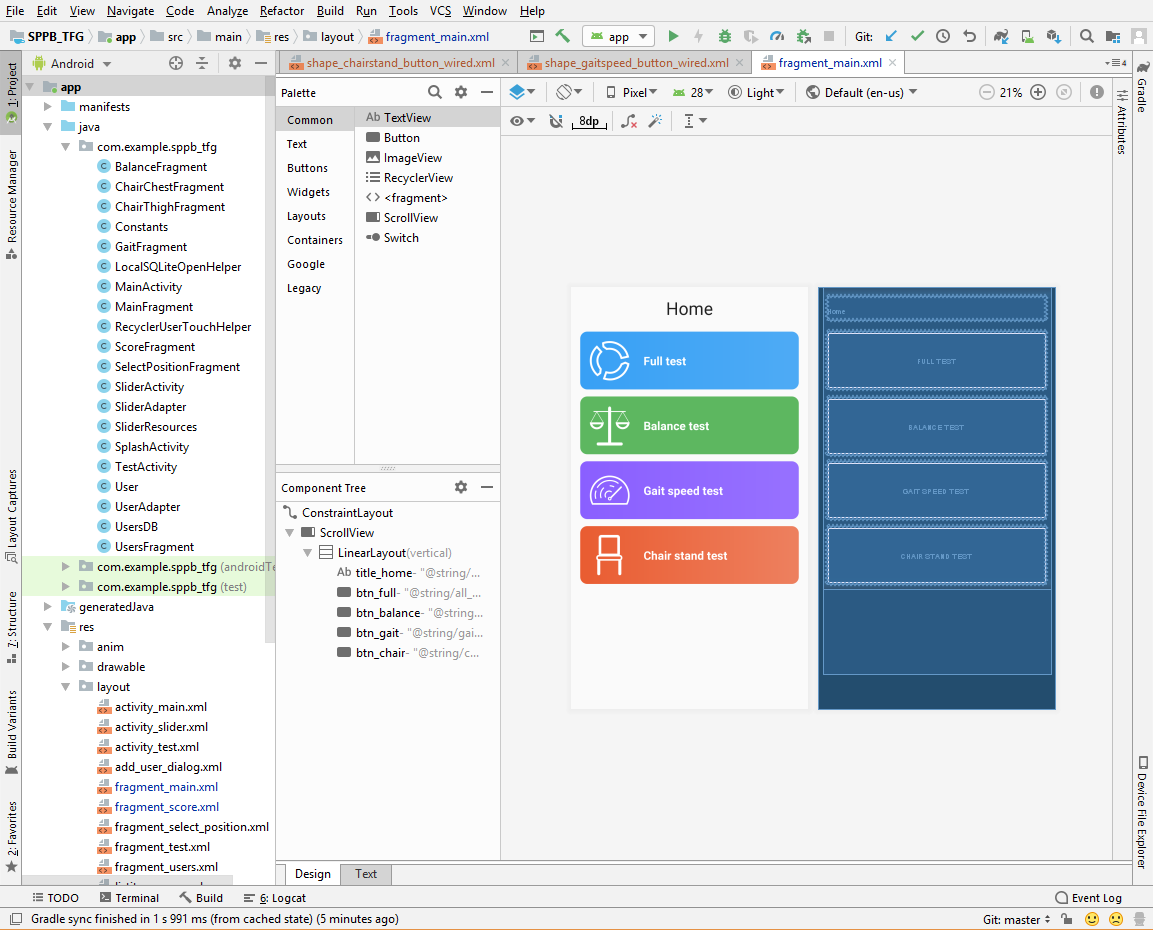
\includegraphics[scale=0.41]{imagenes/android_studio.png}
	\caption{Captura de pantalla de Android Studio\label{fig:android_studio}}
\end{figure}

Puede ser utilizado de forma completamente gratuita en las siguientes plataformas: Microsoft Windows, MacOS y GNU/Linux. Algunas de las principales características con las que cuenta son:
\begin{itemize}
    \item Emulador rápido con distintas funciones.
    \item Herramientas Lint, con la que es posible detectar problemas tales como bajo rendimiento, usabilidad, compatibilidad de versión, etc.
    \item Compatibilidad con C++ y NDK a parte de Java y Kotlin.
    \item Un sistema de compilación Gradle.
    \item Plantillas para los diseños más comunes.
    \item Renderizado en tiempo real.
\end{itemize}

\subsection{Github}
Otra de las herramientas más importantes del proceso ha sido Github. Github es una plataforma de desarrollo colaborativo, especialmente diseñado para alojar proyectos y permitir un control de versiones Git. Cuenta con muchas opciones como la de recuperar cualquier versión pasada del proyecto, indicar qué partes faltan por hacer, cuales están en progreso y cuales han acabado. También es posible comprobar qué usuarios han contribuido al desarrollo de un repositorio\cite{github_wikipedia}.

La principal utilidad que hemos dado a Github en este proyecto ha sido la de crear y mantener una copia de seguridad del código en cada momento, además de facilitar la compartición del mismo con los tutores y mostrarlo de forma pública para quien quiera usarlo, favoreciendo así el desarrollo colaborativo y la filosofía open source.

\subsection{Trello}
Trello es una plataforma online de productividad, enfocada en la gestión de proyectos. Imita a un tablero en donde se colocan notas dentro de diferentes categorías, las cuales pueden ser \textit{Por hacer}, \textit{En proceso} y \textit{Hecho}, entre otras. Además permite y facilita la creación de citas y avisos o el trabajo en equipo\cite{trello}.

\begin{figure}[H]
	\centering
	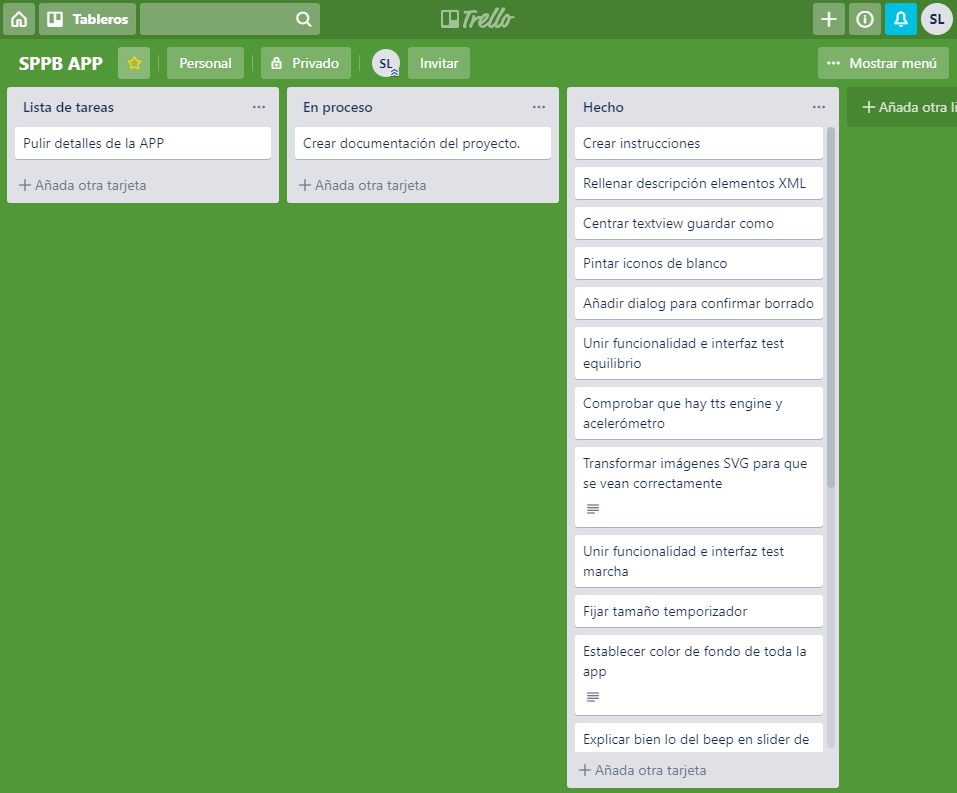
\includegraphics[scale=0.42]{imagenes/trello.png}
	\caption{Captura de pantalla de Trello.com\label{fig:trello}}
\end{figure}

Trello puede ser sustituido por la opción Issues que ofrece Github, puesto que su funcionamiento y cometido son muy similares. No obstante, debido a la gran facilidad de uso, nos hemos decantado por Trello en esta ocasión.